\documentclass[1p]{elsarticle_modified}
%\bibliographystyle{elsarticle-num}

%\usepackage[colorlinks]{hyperref}
%\usepackage{abbrmath_seonhwa} %\Abb, \Ascr, \Acal ,\Abf, \Afrak
\usepackage{amsfonts}
\usepackage{amssymb}
\usepackage{amsmath}
\usepackage{amsthm}
\usepackage{scalefnt}
\usepackage{amsbsy}
\usepackage{kotex}
\usepackage{caption}
\usepackage{subfig}
\usepackage{color}
\usepackage{graphicx}
\usepackage{xcolor} %% white, black, red, green, blue, cyan, magenta, yellow
\usepackage{float}
\usepackage{setspace}
\usepackage{hyperref}

\usepackage{tikz}
\usetikzlibrary{arrows}

\usepackage{multirow}
\usepackage{array} % fixed length table
\usepackage{hhline}

%%%%%%%%%%%%%%%%%%%%%
\makeatletter
\renewcommand*\env@matrix[1][\arraystretch]{%
	\edef\arraystretch{#1}%
	\hskip -\arraycolsep
	\let\@ifnextchar\new@ifnextchar
	\array{*\c@MaxMatrixCols c}}
\makeatother %https://tex.stackexchange.com/questions/14071/how-can-i-increase-the-line-spacing-in-a-matrix
%%%%%%%%%%%%%%%

\usepackage[normalem]{ulem}

\newcommand{\msout}[1]{\ifmmode\text{\sout{\ensuremath{#1}}}\else\sout{#1}\fi}
%SOURCE: \msout is \stkout macro in https://tex.stackexchange.com/questions/20609/strikeout-in-math-mode

\newcommand{\cancel}[1]{
	\ifmmode
	{\color{red}\msout{#1}}
	\else
	{\color{red}\sout{#1}}
	\fi
}

\newcommand{\add}[1]{
	{\color{blue}\uwave{#1}}
}

\newcommand{\replace}[2]{
	\ifmmode
	{\color{red}\msout{#1}}{\color{blue}\uwave{#2}}
	\else
	{\color{red}\sout{#1}}{\color{blue}\uwave{#2}}
	\fi
}

\newcommand{\Sol}{\mathcal{S}} %segment
\newcommand{\D}{D} %diagram
\newcommand{\A}{\mathcal{A}} %arc


%%%%%%%%%%%%%%%%%%%%%%%%%%%%%5 test

\def\sl{\operatorname{\textup{SL}}(2,\Cbb)}
\def\psl{\operatorname{\textup{PSL}}(2,\Cbb)}
\def\quan{\mkern 1mu \triangleright \mkern 1mu}

\theoremstyle{definition}
\newtheorem{thm}{Theorem}[section]
\newtheorem{prop}[thm]{Proposition}
\newtheorem{lem}[thm]{Lemma}
\newtheorem{ques}[thm]{Question}
\newtheorem{cor}[thm]{Corollary}
\newtheorem{defn}[thm]{Definition}
\newtheorem{exam}[thm]{Example}
\newtheorem{rmk}[thm]{Remark}
\newtheorem{alg}[thm]{Algorithm}

\newcommand{\I}{\sqrt{-1}}
\begin{document}

%\begin{frontmatter}
%
%\title{Boundary parabolic representations of knots up to 8 crossings}
%
%%% Group authors per affiliation:
%\author{Yunhi Cho} 
%\address{Department of Mathematics, University of Seoul, Seoul, Korea}
%\ead{yhcho@uos.ac.kr}
%
%
%\author{Seonhwa Kim} %\fnref{s_kim}}
%\address{Center for Geometry and Physics, Institute for Basic Science, Pohang, 37673, Korea}
%\ead{ryeona17@ibs.re.kr}
%
%\author{Hyuk Kim}
%\address{Department of Mathematical Sciences, Seoul National University, Seoul 08826, Korea}
%\ead{hyukkim@snu.ac.kr}
%
%\author{Seokbeom Yoon}
%\address{Department of Mathematical Sciences, Seoul National University, Seoul, 08826,  Korea}
%\ead{sbyoon15@snu.ac.kr}
%
%\begin{abstract}
%We find all boundary parabolic representation of knots up to 8 crossings.
%
%\end{abstract}
%\begin{keyword}
%    \MSC[2010] 57M25 
%\end{keyword}
%
%\end{frontmatter}

%\linenumbers
%\tableofcontents
%
\newcommand\colored[1]{\textcolor{white}{\rule[-0.35ex]{0.8em}{1.4ex}}\kern-0.8em\color{red} #1}%
%\newcommand\colored[1]{\textcolor{white}{ #1}\kern-2.17ex	\textcolor{white}{ #1}\kern-1.81ex	\textcolor{white}{ #1}\kern-2.15ex\color{red}#1	}

{\Large $\underline{11a_{317}~(K11a_{317})}$}

\setlength{\tabcolsep}{10pt}
\renewcommand{\arraystretch}{1.6}
\vspace{1cm}\begin{tabular}{m{100pt}>{\centering\arraybackslash}m{274pt}}
\multirow{5}{120pt}{
	\centering
	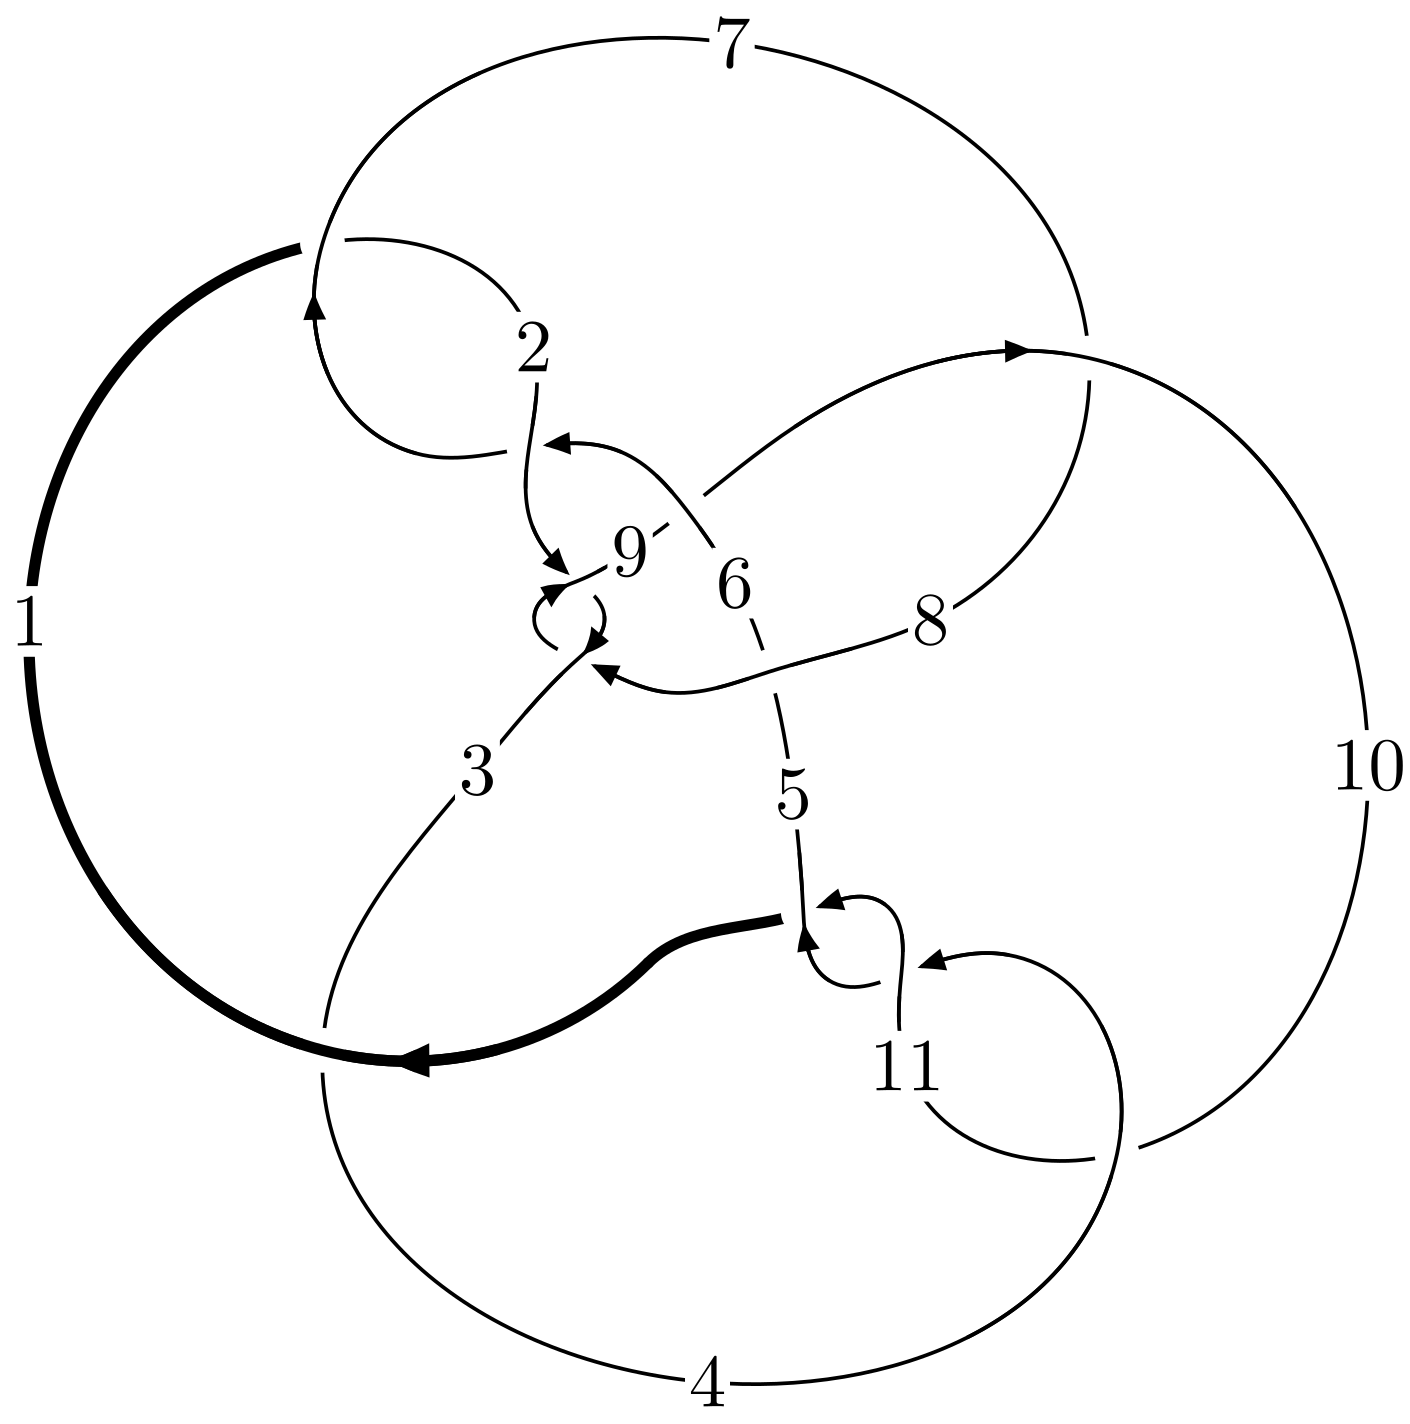
\includegraphics[width=112pt]{../../../GIT/diagram.site/Diagrams/png/566_11a_317.png}\\
\ \ \ A knot diagram\footnotemark}&
\allowdisplaybreaks
\textbf{Linearized knot diagam} \\
\cline{2-2}
 &
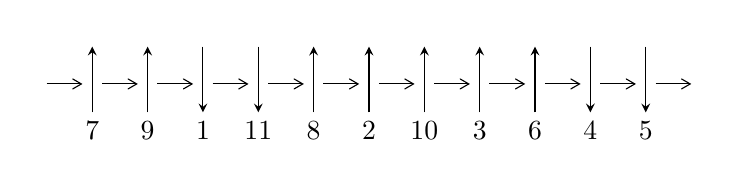
\begin{tikzpicture}[x=20pt, y=17pt]
	% nodes
	\node (C0) at (0, 0) {};
	\node (C1) at (1, 0) {};
	\node (C1U) at (1, +1) {};
	\node (C1D) at (1, -1) {7};

	\node (C2) at (2, 0) {};
	\node (C2U) at (2, +1) {};
	\node (C2D) at (2, -1) {9};

	\node (C3) at (3, 0) {};
	\node (C3U) at (3, +1) {};
	\node (C3D) at (3, -1) {1};

	\node (C4) at (4, 0) {};
	\node (C4U) at (4, +1) {};
	\node (C4D) at (4, -1) {11};

	\node (C5) at (5, 0) {};
	\node (C5U) at (5, +1) {};
	\node (C5D) at (5, -1) {8};

	\node (C6) at (6, 0) {};
	\node (C6U) at (6, +1) {};
	\node (C6D) at (6, -1) {2};

	\node (C7) at (7, 0) {};
	\node (C7U) at (7, +1) {};
	\node (C7D) at (7, -1) {10};

	\node (C8) at (8, 0) {};
	\node (C8U) at (8, +1) {};
	\node (C8D) at (8, -1) {3};

	\node (C9) at (9, 0) {};
	\node (C9U) at (9, +1) {};
	\node (C9D) at (9, -1) {6};

	\node (C10) at (10, 0) {};
	\node (C10U) at (10, +1) {};
	\node (C10D) at (10, -1) {4};

	\node (C11) at (11, 0) {};
	\node (C11U) at (11, +1) {};
	\node (C11D) at (11, -1) {5};
	\node (C12) at (12, 0) {};

	% arrows
	\draw[->,>={angle 60}]
	(C0) edge (C1) (C1) edge (C2) (C2) edge (C3) (C3) edge (C4) (C4) edge (C5) (C5) edge (C6) (C6) edge (C7) (C7) edge (C8) (C8) edge (C9) (C9) edge (C10) (C10) edge (C11) (C11) edge (C12) ;	\draw[->,>=stealth]
	(C1D) edge (C1U) (C2D) edge (C2U) (C3U) edge (C3D) (C4U) edge (C4D) (C5D) edge (C5U) (C6D) edge (C6U) (C7D) edge (C7U) (C8D) edge (C8U) (C9D) edge (C9U) (C10U) edge (C10D) (C11U) edge (C11D) ;
	\end{tikzpicture} \\
\hhline{~~} \\& 
\textbf{Solving Sequence} \\ \cline{2-2} 
 &
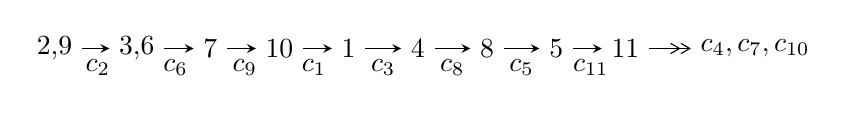
\begin{tikzpicture}[x=25pt, y=7pt]
	% node
	\node (A0) at (-1/8, 0) {2,9};
	\node (A1) at (17/16, 0) {3,6};
	\node (A2) at (17/8, 0) {7};
	\node (A3) at (25/8, 0) {10};
	\node (A4) at (33/8, 0) {1};
	\node (A5) at (41/8, 0) {4};
	\node (A6) at (49/8, 0) {8};
	\node (A7) at (57/8, 0) {5};
	\node (A8) at (65/8, 0) {11};
	\node (C1) at (1/2, -1) {$c_{2}$};
	\node (C2) at (13/8, -1) {$c_{6}$};
	\node (C3) at (21/8, -1) {$c_{9}$};
	\node (C4) at (29/8, -1) {$c_{1}$};
	\node (C5) at (37/8, -1) {$c_{3}$};
	\node (C6) at (45/8, -1) {$c_{8}$};
	\node (C7) at (53/8, -1) {$c_{5}$};
	\node (C8) at (61/8, -1) {$c_{11}$};
	\node (A9) at (10, 0) {$c_{4},c_{7},c_{10}$};

	% edge
	\draw[->,>=stealth]	
	(A0) edge (A1) (A1) edge (A2) (A2) edge (A3) (A3) edge (A4) (A4) edge (A5) (A5) edge (A6) (A6) edge (A7) (A7) edge (A8) ;
	\draw[->>,>={angle 60}]	
	(A8) edge (A9);
\end{tikzpicture} \\ 

\end{tabular} \\

\footnotetext{
The image of knot diagram is generated by the software ``\textbf{Draw programme}" developed by Andrew Bartholomew(\url{http://www.layer8.co.uk/maths/draw/index.htm\#Running-draw}), where we modified some parts for our purpose(\url{https://github.com/CATsTAILs/LinksPainter}).
}\phantom \\ \newline 
\centering \textbf{Ideals for irreducible components\footnotemark of $X_{\text{par}}$} 
 
\begin{align*}
I^u_{1}&=\langle 
b- u,\;9521222 u^{24}+7310497 u^{23}+\cdots+51467938 a+84913603,\;u^{25}+9 u^{23}+\cdots+2 u-1\rangle \\
I^u_{2}&=\langle 
-3.79702\times10^{56} u^{47}-2.02674\times10^{55} u^{46}+\cdots+3.40179\times10^{58} b+1.47690\times10^{59},\\
\phantom{I^u_{2}}&\phantom{= \langle  }-2.59043\times10^{36} u^{47}-5.89061\times10^{36} u^{46}+\cdots+8.97537\times10^{37} a-1.46834\times10^{39},\\
\phantom{I^u_{2}}&\phantom{= \langle  }u^{48}+u^{47}+\cdots-114 u+76\rangle \\
I^u_{3}&=\langle 
b+u,\;- u^8-5 u^6- u^5-10 u^4-3 u^3-9 u^2+a-3 u-3,\\
\phantom{I^u_{3}}&\phantom{= \langle  }u^{11}+6 u^9+u^8+15 u^7+4 u^6+19 u^5+6 u^4+12 u^3+3 u^2+3 u+1\rangle \\
\\
\end{align*}
\raggedright * 3 irreducible components of $\dim_{\mathbb{C}}=0$, with total 84 representations.\\
\footnotetext{All coefficients of polynomials are rational numbers. But the coefficients are sometimes approximated in decimal forms when there is not enough margin.}
\newpage
\renewcommand{\arraystretch}{1}
\centering \section*{I. $I^u_{1}= \langle b- u,\;9.52\times10^{6} u^{24}+7.31\times10^{6} u^{23}+\cdots+5.15\times10^{7} a+8.49\times10^{7},\;u^{25}+9 u^{23}+\cdots+2 u-1 \rangle$}
\flushleft \textbf{(i) Arc colorings}\\
\begin{tabular}{m{7pt} m{180pt} m{7pt} m{180pt} }
\flushright $a_{2}=$&$\begin{pmatrix}1\\0\end{pmatrix}$ \\
\flushright $a_{9}=$&$\begin{pmatrix}0\\u\end{pmatrix}$ \\
\flushright $a_{3}=$&$\begin{pmatrix}1\\- u^2\end{pmatrix}$ \\
\flushright $a_{6}=$&$\begin{pmatrix}-0.184993 u^{24}-0.142040 u^{23}+\cdots+0.533191 u-1.64983\\u\end{pmatrix}$ \\
\flushright $a_{7}=$&$\begin{pmatrix}-0.184993 u^{24}-0.142040 u^{23}+\cdots+1.53319 u-1.64983\\u\end{pmatrix}$ \\
\flushright $a_{10}=$&$\begin{pmatrix}0.249484 u^{24}+0.573176 u^{23}+\cdots-1.83450 u+1.36074\\-0.208863 u^{24}-0.229234 u^{23}+\cdots+1.09909 u-0.142040\end{pmatrix}$ \\
\flushright $a_{1}=$&$\begin{pmatrix}-0.142040 u^{24}-0.208863 u^{23}+\cdots-1.27985 u+0.815007\\u^2\end{pmatrix}$ \\
\flushright $a_{4}=$&$\begin{pmatrix}-0.404984 u^{24}-0.142520 u^{23}+\cdots-0.371512 u+1.03005\\0.127693 u^{24}-0.0749250 u^{23}+\cdots-0.532638 u+0.151702\end{pmatrix}$ \\
\flushright $a_{8}=$&$\begin{pmatrix}- u\\u^3+u\end{pmatrix}$ \\
\flushright $a_{5}=$&$\begin{pmatrix}-0.127833 u^{24}-0.0404991 u^{23}+\cdots+0.184500 u-1.27856\\0.0196164 u^{24}+0.173697 u^{23}+\cdots+1.49461 u-0.472814\end{pmatrix}$ \\
\flushright $a_{11}=$&$\begin{pmatrix}-0.127434 u^{24}+0.297945 u^{23}+\cdots-1.85707 u+1.03254\\-0.293850 u^{24}-0.0592649 u^{23}+\cdots+1.55630 u-0.291252\end{pmatrix}$\\ \flushright $a_{11}=$&$\begin{pmatrix}-0.127434 u^{24}+0.297945 u^{23}+\cdots-1.85707 u+1.03254\\-0.293850 u^{24}-0.0592649 u^{23}+\cdots+1.55630 u-0.291252\end{pmatrix}$\\&\end{tabular}
\flushleft \textbf{(ii) Obstruction class $= -1$}\\~\\
\flushleft \textbf{(iii) Cusp Shapes $= \frac{82053183}{25733969} u^{24}+\frac{57865173}{25733969} u^{23}+\cdots-\frac{4551724}{25733969} u+\frac{217825726}{25733969}$}\\~\\
\newpage\renewcommand{\arraystretch}{1}
\flushleft \textbf{(iv) u-Polynomials at the component}\newline \\
\begin{tabular}{m{50pt}|m{274pt}}
Crossings & \hspace{64pt}u-Polynomials at each crossing \\
\hline $$\begin{aligned}c_{1},c_{2},c_{6}\\c_{8}\end{aligned}$$&$\begin{aligned}
&u^{25}+9 u^{23}+\cdots+2 u-1
\end{aligned}$\\
\hline $$\begin{aligned}c_{3}\end{aligned}$$&$\begin{aligned}
&u^{25}-18 u^{24}+\cdots+1946 u-188
\end{aligned}$\\
\hline $$\begin{aligned}c_{4},c_{10},c_{11}\end{aligned}$$&$\begin{aligned}
&u^{25}+6 u^{24}+\cdots+14 u-4
\end{aligned}$\\
\hline $$\begin{aligned}c_{5},c_{7}\end{aligned}$$&$\begin{aligned}
&u^{25}- u^{24}+\cdots-3 u-1
\end{aligned}$\\
\hline $$\begin{aligned}c_{9}\end{aligned}$$&$\begin{aligned}
&u^{25}-23 u^{24}+\cdots+49152 u-4096
\end{aligned}$\\
\hline
\end{tabular}\\~\\
\newpage\renewcommand{\arraystretch}{1}
\flushleft \textbf{(v) Riley Polynomials at the component}\newline \\
\begin{tabular}{m{50pt}|m{274pt}}
Crossings & \hspace{64pt}Riley Polynomials at each crossing \\
\hline $$\begin{aligned}c_{1},c_{2},c_{6}\\c_{8}\end{aligned}$$&$\begin{aligned}
&y^{25}+18 y^{24}+\cdots+4 y-1
\end{aligned}$\\
\hline $$\begin{aligned}c_{3}\end{aligned}$$&$\begin{aligned}
&y^{25}+2 y^{24}+\cdots+360428 y-35344
\end{aligned}$\\
\hline $$\begin{aligned}c_{4},c_{10},c_{11}\end{aligned}$$&$\begin{aligned}
&y^{25}-22 y^{24}+\cdots+140 y-16
\end{aligned}$\\
\hline $$\begin{aligned}c_{5},c_{7}\end{aligned}$$&$\begin{aligned}
&y^{25}-5 y^{24}+\cdots+19 y-1
\end{aligned}$\\
\hline $$\begin{aligned}c_{9}\end{aligned}$$&$\begin{aligned}
&y^{25}- y^{24}+\cdots+25165824 y-16777216
\end{aligned}$\\
\hline
\end{tabular}\\~\\
\newpage\flushleft \textbf{(vi) Complex Volumes and Cusp Shapes}
$$\begin{array}{c|c|c}  
\text{Solutions to }I^u_{1}& \I (\text{vol} + \sqrt{-1}CS) & \text{Cusp shape}\\
 \hline 
\begin{aligned}
u &= -0.062688 + 1.054190 I \\
a &= -0.22875 + 2.02308 I \\
b &= -0.062688 + 1.054190 I\end{aligned}
 & -1.10259 - 2.56061 I & \phantom{-}2.13530 + 4.85725 I \\ \hline\begin{aligned}
u &= -0.062688 - 1.054190 I \\
a &= -0.22875 - 2.02308 I \\
b &= -0.062688 - 1.054190 I\end{aligned}
 & -1.10259 + 2.56061 I & \phantom{-}2.13530 - 4.85725 I \\ \hline\begin{aligned}
u &= -0.431005 + 1.014420 I \\
a &= \phantom{-}1.57469 - 0.29419 I \\
b &= -0.431005 + 1.014420 I\end{aligned}
 & -3.98322 - 6.30520 I & \phantom{-}2.04460 + 8.85471 I \\ \hline\begin{aligned}
u &= -0.431005 - 1.014420 I \\
a &= \phantom{-}1.57469 + 0.29419 I \\
b &= -0.431005 - 1.014420 I\end{aligned}
 & -3.98322 + 6.30520 I & \phantom{-}2.04460 - 8.85471 I \\ \hline\begin{aligned}
u &= \phantom{-}0.111664 + 1.150710 I \\
a &= \phantom{-}0.55005 + 1.77135 I \\
b &= \phantom{-}0.111664 + 1.150710 I\end{aligned}
 & -7.45610 + 6.63321 I & -3.37442 - 6.60504 I \\ \hline\begin{aligned}
u &= \phantom{-}0.111664 - 1.150710 I \\
a &= \phantom{-}0.55005 - 1.77135 I \\
b &= \phantom{-}0.111664 - 1.150710 I\end{aligned}
 & -7.45610 - 6.63321 I & -3.37442 + 6.60504 I \\ \hline\begin{aligned}
u &= \phantom{-}0.817149 + 0.195179 I \\
a &= -0.818471 + 0.839836 I \\
b &= \phantom{-}0.817149 + 0.195179 I\end{aligned}
 & -1.75933 - 5.22873 I & \phantom{-}2.70405 + 4.29469 I \\ \hline\begin{aligned}
u &= \phantom{-}0.817149 - 0.195179 I \\
a &= -0.818471 - 0.839836 I \\
b &= \phantom{-}0.817149 - 0.195179 I\end{aligned}
 & -1.75933 + 5.22873 I & \phantom{-}2.70405 - 4.29469 I \\ \hline\begin{aligned}
u &= \phantom{-}0.329284 + 0.707437 I \\
a &= -1.12449 - 1.00862 I \\
b &= \phantom{-}0.329284 + 0.707437 I\end{aligned}
 & \phantom{-}0.24887 + 1.85876 I & \phantom{-}5.21169 - 1.18731 I \\ \hline\begin{aligned}
u &= \phantom{-}0.329284 - 0.707437 I \\
a &= -1.12449 + 1.00862 I \\
b &= \phantom{-}0.329284 - 0.707437 I\end{aligned}
 & \phantom{-}0.24887 - 1.85876 I & \phantom{-}5.21169 + 1.18731 I\\
 \hline 
 \end{array}$$\newpage$$\begin{array}{c|c|c}  
\text{Solutions to }I^u_{1}& \I (\text{vol} + \sqrt{-1}CS) & \text{Cusp shape}\\
 \hline 
\begin{aligned}
u &= -0.682331 + 0.261986 I \\
a &= \phantom{-}0.916549 + 0.989308 I \\
b &= -0.682331 + 0.261986 I\end{aligned}
 & \phantom{-}2.97560 + 1.99862 I & \phantom{-}9.19617 - 1.79116 I \\ \hline\begin{aligned}
u &= -0.682331 - 0.261986 I \\
a &= \phantom{-}0.916549 - 0.989308 I \\
b &= -0.682331 - 0.261986 I\end{aligned}
 & \phantom{-}2.97560 - 1.99862 I & \phantom{-}9.19617 + 1.79116 I \\ \hline\begin{aligned}
u &= -0.650446 + 0.309358 I \\
a &= \phantom{-}0.859033 - 0.557233 I \\
b &= -0.650446 + 0.309358 I\end{aligned}
 & -2.96955 + 0.98970 I & \phantom{-}0.58497 + 1.31216 I \\ \hline\begin{aligned}
u &= -0.650446 - 0.309358 I \\
a &= \phantom{-}0.859033 + 0.557233 I \\
b &= -0.650446 - 0.309358 I\end{aligned}
 & -2.96955 - 0.98970 I & \phantom{-}0.58497 - 1.31216 I \\ \hline\begin{aligned}
u &= \phantom{-}0.506874 + 0.472329 I \\
a &= -0.77448 + 1.43912 I \\
b &= \phantom{-}0.506874 + 0.472329 I\end{aligned}
 & \phantom{-}0.027101 + 0.899324 I & \phantom{-}2.44779 - 5.98780 I \\ \hline\begin{aligned}
u &= \phantom{-}0.506874 - 0.472329 I \\
a &= -0.77448 - 1.43912 I \\
b &= \phantom{-}0.506874 - 0.472329 I\end{aligned}
 & \phantom{-}0.027101 - 0.899324 I & \phantom{-}2.44779 + 5.98780 I \\ \hline\begin{aligned}
u &= \phantom{-}0.343162 + 1.368570 I \\
a &= -1.274410 + 0.462559 I \\
b &= \phantom{-}0.343162 + 1.368570 I\end{aligned}
 & -13.7635 + 5.7019 I & -6.58533 - 4.59320 I \\ \hline\begin{aligned}
u &= \phantom{-}0.343162 - 1.368570 I \\
a &= -1.274410 - 0.462559 I \\
b &= \phantom{-}0.343162 - 1.368570 I\end{aligned}
 & -13.7635 - 5.7019 I & -6.58533 + 4.59320 I \\ \hline\begin{aligned}
u &= -0.49075 + 1.33946 I \\
a &= \phantom{-}1.212400 + 0.228564 I \\
b &= -0.49075 + 1.33946 I\end{aligned}
 & -5.95198 - 7.41816 I & -1.58248 + 3.87242 I \\ \hline\begin{aligned}
u &= -0.49075 - 1.33946 I \\
a &= \phantom{-}1.212400 - 0.228564 I \\
b &= -0.49075 - 1.33946 I\end{aligned}
 & -5.95198 + 7.41816 I & -1.58248 - 3.87242 I\\
 \hline 
 \end{array}$$\newpage$$\begin{array}{c|c|c}  
\text{Solutions to }I^u_{1}& \I (\text{vol} + \sqrt{-1}CS) & \text{Cusp shape}\\
 \hline 
\begin{aligned}
u &= \phantom{-}0.54170 + 1.40648 I \\
a &= -1.106250 + 0.225454 I \\
b &= \phantom{-}0.54170 + 1.40648 I\end{aligned}
 & -4.43838 + 12.03070 I & \phantom{-}0.63983 - 8.03648 I \\ \hline\begin{aligned}
u &= \phantom{-}0.54170 - 1.40648 I \\
a &= -1.106250 - 0.225454 I \\
b &= \phantom{-}0.54170 - 1.40648 I\end{aligned}
 & -4.43838 - 12.03070 I & \phantom{-}0.63983 + 8.03648 I \\ \hline\begin{aligned}
u &= -0.54820 + 1.46070 I \\
a &= \phantom{-}1.052770 + 0.249978 I \\
b &= -0.54820 + 1.46070 I\end{aligned}
 & -10.0254 - 16.0606 I & -3.24174 + 8.45261 I \\ \hline\begin{aligned}
u &= -0.54820 - 1.46070 I \\
a &= \phantom{-}1.052770 - 0.249978 I \\
b &= -0.54820 - 1.46070 I\end{aligned}
 & -10.0254 + 16.0606 I & -3.24174 - 8.45261 I \\ \hline\begin{aligned}
u &= \phantom{-}0.431188\phantom{ +0.000000I} \\
a &= -1.67732\phantom{ +0.000000I} \\
b &= \phantom{-}0.431188\phantom{ +0.000000I}\end{aligned}
 & \phantom{-}0.990720\phantom{ +0.000000I} & \phantom{-}10.6390\phantom{ +0.000000I}\\
 \hline 
 \end{array}$$\newpage\newpage\renewcommand{\arraystretch}{1}
\centering \section*{II. $I^u_{2}= \langle -3.80\times10^{56} u^{47}-2.03\times10^{55} u^{46}+\cdots+3.40\times10^{58} b+1.48\times10^{59},\;-2.59\times10^{36} u^{47}-5.89\times10^{36} u^{46}+\cdots+8.98\times10^{37} a-1.47\times10^{39},\;u^{48}+u^{47}+\cdots-114 u+76 \rangle$}
\flushleft \textbf{(i) Arc colorings}\\
\begin{tabular}{m{7pt} m{180pt} m{7pt} m{180pt} }
\flushright $a_{2}=$&$\begin{pmatrix}1\\0\end{pmatrix}$ \\
\flushright $a_{9}=$&$\begin{pmatrix}0\\u\end{pmatrix}$ \\
\flushright $a_{3}=$&$\begin{pmatrix}1\\- u^2\end{pmatrix}$ \\
\flushright $a_{6}=$&$\begin{pmatrix}0.0288615 u^{47}+0.0656308 u^{46}+\cdots-20.8449 u+16.3597\\0.0111618 u^{47}+0.000595787 u^{46}+\cdots+9.23632 u-4.34154\end{pmatrix}$ \\
\flushright $a_{7}=$&$\begin{pmatrix}0.0400233 u^{47}+0.0662266 u^{46}+\cdots-11.6086 u+12.0181\\0.0111618 u^{47}+0.000595787 u^{46}+\cdots+9.23632 u-4.34154\end{pmatrix}$ \\
\flushright $a_{10}=$&$\begin{pmatrix}0.0420194 u^{47}+0.0787887 u^{46}+\cdots-0.594941 u+14.8597\\0.111068 u^{47}+0.0434318 u^{46}+\cdots+17.5888 u-7.60663\end{pmatrix}$ \\
\flushright $a_{1}=$&$\begin{pmatrix}0.0168138 u^{47}+0.0776572 u^{46}+\cdots+24.0640 u+0.627739\\-0.0832734 u^{47}-0.133498 u^{46}+\cdots-8.45658 u-5.55110\end{pmatrix}$ \\
\flushright $a_{4}=$&$\begin{pmatrix}-0.145940 u^{47}+0.0918329 u^{46}+\cdots-59.0154 u+24.9472\\-0.101135 u^{47}+0.0935008 u^{46}+\cdots-8.22727 u+14.4058\end{pmatrix}$ \\
\flushright $a_{8}=$&$\begin{pmatrix}- u\\u^3+u\end{pmatrix}$ \\
\flushright $a_{5}=$&$\begin{pmatrix}0.0201071 u^{47}+0.104301 u^{46}+\cdots-26.0937 u+18.7558\\0.00804912 u^{47}+0.0333014 u^{46}+\cdots+8.41343 u-3.13339\end{pmatrix}$ \\
\flushright $a_{11}=$&$\begin{pmatrix}0.106068 u^{47}+0.361549 u^{46}+\cdots+20.9043 u+2.41440\\-0.0231108 u^{47}+0.124603 u^{46}+\cdots-30.6445 u+6.90238\end{pmatrix}$\\ \flushright $a_{11}=$&$\begin{pmatrix}0.106068 u^{47}+0.361549 u^{46}+\cdots+20.9043 u+2.41440\\-0.0231108 u^{47}+0.124603 u^{46}+\cdots-30.6445 u+6.90238\end{pmatrix}$\\&\end{tabular}
\flushleft \textbf{(ii) Obstruction class $= -1$}\\~\\
\flushleft \textbf{(iii) Cusp Shapes $= -0.299258 u^{47}-0.246468 u^{46}+\cdots+7.59368 u-10.2839$}\\~\\
\newpage\renewcommand{\arraystretch}{1}
\flushleft \textbf{(iv) u-Polynomials at the component}\newline \\
\begin{tabular}{m{50pt}|m{274pt}}
Crossings & \hspace{64pt}u-Polynomials at each crossing \\
\hline $$\begin{aligned}c_{1},c_{2},c_{6}\\c_{8}\end{aligned}$$&$\begin{aligned}
&u^{48}+u^{47}+\cdots-114 u+76
\end{aligned}$\\
\hline $$\begin{aligned}c_{3}\end{aligned}$$&$\begin{aligned}
&(u^{12}+3 u^{11}+\cdots+4 u+1)^{4}
\end{aligned}$\\
\hline $$\begin{aligned}c_{4},c_{10},c_{11}\end{aligned}$$&$\begin{aligned}
&(u^{12}- u^{11}-5 u^{10}+4 u^9+9 u^8-4 u^7-6 u^6-2 u^5+3 u^3+u^2+1)^4
\end{aligned}$\\
\hline $$\begin{aligned}c_{5},c_{7}\end{aligned}$$&$\begin{aligned}
&u^{48}+13 u^{47}+\cdots+54 u+4
\end{aligned}$\\
\hline $$\begin{aligned}c_{9}\end{aligned}$$&$\begin{aligned}
&(u^2+u+1)^{24}
\end{aligned}$\\
\hline
\end{tabular}\\~\\
\newpage\renewcommand{\arraystretch}{1}
\flushleft \textbf{(v) Riley Polynomials at the component}\newline \\
\begin{tabular}{m{50pt}|m{274pt}}
Crossings & \hspace{64pt}Riley Polynomials at each crossing \\
\hline $$\begin{aligned}c_{1},c_{2},c_{6}\\c_{8}\end{aligned}$$&$\begin{aligned}
&y^{48}+39 y^{47}+\cdots+220932 y+5776
\end{aligned}$\\
\hline $$\begin{aligned}c_{3}\end{aligned}$$&$\begin{aligned}
&(y^{12}+y^{11}+\cdots-2 y+1)^{4}
\end{aligned}$\\
\hline $$\begin{aligned}c_{4},c_{10},c_{11}\end{aligned}$$&$\begin{aligned}
&(y^{12}-11 y^{11}+\cdots+2 y+1)^{4}
\end{aligned}$\\
\hline $$\begin{aligned}c_{5},c_{7}\end{aligned}$$&$\begin{aligned}
&y^{48}+11 y^{47}+\cdots+356 y+16
\end{aligned}$\\
\hline $$\begin{aligned}c_{9}\end{aligned}$$&$\begin{aligned}
&(y^2+y+1)^{24}
\end{aligned}$\\
\hline
\end{tabular}\\~\\
\newpage\flushleft \textbf{(vi) Complex Volumes and Cusp Shapes}
$$\begin{array}{c|c|c}  
\text{Solutions to }I^u_{2}& \I (\text{vol} + \sqrt{-1}CS) & \text{Cusp shape}\\
 \hline 
\begin{aligned}
u &= \phantom{-}0.119725 + 0.978589 I \\
a &= \phantom{-}0.933512 - 0.396730 I \\
b &= -0.735953 + 0.216627 I\end{aligned}
 & -1.81971 + 1.93627 I & -0.00912 - 4.22614 I \\ \hline\begin{aligned}
u &= \phantom{-}0.119725 - 0.978589 I \\
a &= \phantom{-}0.933512 + 0.396730 I \\
b &= -0.735953 - 0.216627 I\end{aligned}
 & -1.81971 - 1.93627 I & -0.00912 + 4.22614 I \\ \hline\begin{aligned}
u &= -0.975387 + 0.053637 I \\
a &= -0.462394 - 0.913306 I \\
b &= \phantom{-}0.248414 + 1.077640 I\end{aligned}
 & -1.81971 + 2.12349 I & -0.00912 - 2.70206 I \\ \hline\begin{aligned}
u &= -0.975387 - 0.053637 I \\
a &= -0.462394 + 0.913306 I \\
b &= \phantom{-}0.248414 - 1.077640 I\end{aligned}
 & -1.81971 - 2.12349 I & -0.00912 + 2.70206 I \\ \hline\begin{aligned}
u &= \phantom{-}0.248414 + 1.077640 I \\
a &= \phantom{-}0.864641 - 0.264663 I \\
b &= -0.975387 + 0.053637 I\end{aligned}
 & -1.81971 + 2.12349 I & \phantom{-0.000000 } 0. - 2.70206 I \\ \hline\begin{aligned}
u &= \phantom{-}0.248414 - 1.077640 I \\
a &= \phantom{-}0.864641 + 0.264663 I \\
b &= -0.975387 - 0.053637 I\end{aligned}
 & -1.81971 - 2.12349 I & \phantom{-0.000000 -}0. + 2.70206 I \\ \hline\begin{aligned}
u &= \phantom{-}0.423066 + 0.782946 I \\
a &= -0.589046 - 0.956905 I \\
b &= \phantom{-}0.087660 + 0.519316 I\end{aligned}
 & \phantom{-}0.20418 + 1.85492 I & \phantom{-}2.80561 - 0.70730 I \\ \hline\begin{aligned}
u &= \phantom{-}0.423066 - 0.782946 I \\
a &= -0.589046 + 0.956905 I \\
b &= \phantom{-}0.087660 - 0.519316 I\end{aligned}
 & \phantom{-}0.20418 - 1.85492 I & \phantom{-}2.80561 + 0.70730 I \\ \hline\begin{aligned}
u &= \phantom{-}0.839580 + 0.740780 I \\
a &= \phantom{-}0.846588 + 0.284535 I \\
b &= -0.200259 - 1.354980 I\end{aligned}
 & -8.04990 + 1.93627 I & -3.99088 - 4.22614 I \\ \hline\begin{aligned}
u &= \phantom{-}0.839580 - 0.740780 I \\
a &= \phantom{-}0.846588 - 0.284535 I \\
b &= -0.200259 + 1.354980 I\end{aligned}
 & -8.04990 - 1.93627 I & -3.99088 + 4.22614 I\\
 \hline 
 \end{array}$$\newpage$$\begin{array}{c|c|c}  
\text{Solutions to }I^u_{2}& \I (\text{vol} + \sqrt{-1}CS) & \text{Cusp shape}\\
 \hline 
\begin{aligned}
u &= -0.103555 + 1.115340 I \\
a &= -0.811099 - 0.372987 I \\
b &= \phantom{-}0.42519 - 1.56466 I\end{aligned}
 & -4.93480 - 0.82777 I & -2.00000 - 2.17330 I \\ \hline\begin{aligned}
u &= -0.103555 - 1.115340 I \\
a &= -0.811099 + 0.372987 I \\
b &= \phantom{-}0.42519 + 1.56466 I\end{aligned}
 & -4.93480 + 0.82777 I & -2.00000 + 2.17330 I \\ \hline\begin{aligned}
u &= -0.021432 + 1.150630 I \\
a &= \phantom{-}0.744302 - 0.448409 I \\
b &= -0.49671 - 1.71193 I\end{aligned}
 & -10.07380 - 1.85492 I & -6.80561 + 0.70730 I \\ \hline\begin{aligned}
u &= -0.021432 - 1.150630 I \\
a &= \phantom{-}0.744302 + 0.448409 I \\
b &= -0.49671 + 1.71193 I\end{aligned}
 & -10.07380 + 1.85492 I & -6.80561 - 0.70730 I \\ \hline\begin{aligned}
u &= -0.531251 + 1.069240 I \\
a &= \phantom{-}0.463250 - 0.697786 I \\
b &= \phantom{-}0.089046 + 0.280790 I\end{aligned}
 & -4.93480 - 5.55830 I & -2.00000 + 1.67128 I \\ \hline\begin{aligned}
u &= -0.531251 - 1.069240 I \\
a &= \phantom{-}0.463250 + 0.697786 I \\
b &= \phantom{-}0.089046 - 0.280790 I\end{aligned}
 & -4.93480 + 5.55830 I & -2.00000 - 1.67128 I \\ \hline\begin{aligned}
u &= -0.358210 + 1.155170 I \\
a &= -0.806376 - 0.182786 I \\
b &= \phantom{-}1.230640 - 0.061737 I\end{aligned}
 & \phantom{-}0.20418 - 5.91469 I & \phantom{-}3.00000 + 7.63550 I \\ \hline\begin{aligned}
u &= -0.358210 - 1.155170 I \\
a &= -0.806376 + 0.182786 I \\
b &= \phantom{-}1.230640 + 0.061737 I\end{aligned}
 & \phantom{-}0.20418 + 5.91469 I & \phantom{-}3.00000 - 7.63550 I \\ \hline\begin{aligned}
u &= \phantom{-}1.230640 + 0.061737 I \\
a &= \phantom{-}0.440487 + 0.681622 I \\
b &= -0.358210 - 1.155170 I\end{aligned}
 & \phantom{-}0.20418 + 5.91469 I & \phantom{-}3.00000 - 7.63550 I \\ \hline\begin{aligned}
u &= \phantom{-}1.230640 - 0.061737 I \\
a &= \phantom{-}0.440487 - 0.681622 I \\
b &= -0.358210 + 1.155170 I\end{aligned}
 & \phantom{-}0.20418 - 5.91469 I & \phantom{-}3.00000 + 7.63550 I\\
 \hline 
 \end{array}$$\newpage$$\begin{array}{c|c|c}  
\text{Solutions to }I^u_{2}& \I (\text{vol} + \sqrt{-1}CS) & \text{Cusp shape}\\
 \hline 
\begin{aligned}
u &= -0.735953 + 0.216627 I \\
a &= -0.306466 - 1.266950 I \\
b &= \phantom{-}0.119725 + 0.978589 I\end{aligned}
 & -1.81971 + 1.93627 I & -0.00912 - 4.22614 I \\ \hline\begin{aligned}
u &= -0.735953 - 0.216627 I \\
a &= -0.306466 + 1.266950 I \\
b &= \phantom{-}0.119725 - 0.978589 I\end{aligned}
 & -1.81971 - 1.93627 I & -0.00912 + 4.22614 I \\ \hline\begin{aligned}
u &= \phantom{-}0.393376 + 1.207210 I \\
a &= \phantom{-}0.770526 - 0.163098 I \\
b &= -1.341440 - 0.149230 I\end{aligned}
 & -4.93480 + 9.61806 I & \phantom{-0.000000 } 0. - 8.59949 I \\ \hline\begin{aligned}
u &= \phantom{-}0.393376 - 1.207210 I \\
a &= \phantom{-}0.770526 + 0.163098 I \\
b &= -1.341440 + 0.149230 I\end{aligned}
 & -4.93480 - 9.61806 I & \phantom{-0.000000 -}0. + 8.59949 I \\ \hline\begin{aligned}
u &= \phantom{-}0.139190 + 1.313850 I \\
a &= \phantom{-}0.691702 - 0.307281 I \\
b &= -0.68913 - 1.36774 I\end{aligned}
 & -4.93480 + 3.23200 I & \phantom{-0.000000 } 0 \\ \hline\begin{aligned}
u &= \phantom{-}0.139190 - 1.313850 I \\
a &= \phantom{-}0.691702 + 0.307281 I \\
b &= -0.68913 + 1.36774 I\end{aligned}
 & -4.93480 - 3.23200 I & \phantom{-0.000000 } 0 \\ \hline\begin{aligned}
u &= -0.068128 + 1.345270 I \\
a &= -0.660883 - 0.338204 I \\
b &= \phantom{-}0.81330 - 1.51334 I\end{aligned}
 & -10.07380 - 5.91469 I & \phantom{-0.000000 } 0 \\ \hline\begin{aligned}
u &= -0.068128 - 1.345270 I \\
a &= -0.660883 + 0.338204 I \\
b &= \phantom{-}0.81330 + 1.51334 I\end{aligned}
 & -10.07380 + 5.91469 I & \phantom{-0.000000 } 0 \\ \hline\begin{aligned}
u &= \phantom{-}0.280065 + 0.589338 I \\
a &= \phantom{-}1.52767 - 0.12243 I \\
b &= -0.06781 - 1.45011 I\end{aligned}
 & -8.04990 + 2.12349 I & -3.99088 - 2.70206 I \\ \hline\begin{aligned}
u &= \phantom{-}0.280065 - 0.589338 I \\
a &= \phantom{-}1.52767 + 0.12243 I \\
b &= -0.06781 + 1.45011 I\end{aligned}
 & -8.04990 - 2.12349 I & -3.99088 + 2.70206 I\\
 \hline 
 \end{array}$$\newpage$$\begin{array}{c|c|c}  
\text{Solutions to }I^u_{2}& \I (\text{vol} + \sqrt{-1}CS) & \text{Cusp shape}\\
 \hline 
\begin{aligned}
u &= -1.341440 + 0.149230 I \\
a &= -0.439121 + 0.596745 I \\
b &= \phantom{-}0.393376 - 1.207210 I\end{aligned}
 & -4.93480 - 9.61806 I & \phantom{-0.000000 } 0 \\ \hline\begin{aligned}
u &= -1.341440 - 0.149230 I \\
a &= -0.439121 - 0.596745 I \\
b &= \phantom{-}0.393376 + 1.207210 I\end{aligned}
 & -4.93480 + 9.61806 I & \phantom{-0.000000 } 0 \\ \hline\begin{aligned}
u &= -0.200259 + 1.354980 I \\
a &= -0.678850 - 0.268678 I \\
b &= \phantom{-}0.839580 - 0.740780 I\end{aligned}
 & -8.04990 - 1.93627 I & \phantom{-0.000000 } 0 \\ \hline\begin{aligned}
u &= -0.200259 - 1.354980 I \\
a &= -0.678850 + 0.268678 I \\
b &= \phantom{-}0.839580 + 0.740780 I\end{aligned}
 & -8.04990 + 1.93627 I & \phantom{-0.000000 } 0 \\ \hline\begin{aligned}
u &= -0.06781 + 1.45011 I \\
a &= -0.612000 - 0.316184 I \\
b &= \phantom{-}0.280065 - 0.589338 I\end{aligned}
 & -8.04990 - 2.12349 I & \phantom{-0.000000 } 0 \\ \hline\begin{aligned}
u &= -0.06781 - 1.45011 I \\
a &= -0.612000 + 0.316184 I \\
b &= \phantom{-}0.280065 + 0.589338 I\end{aligned}
 & -8.04990 + 2.12349 I & \phantom{-0.000000 } 0 \\ \hline\begin{aligned}
u &= \phantom{-}0.087660 + 0.519316 I \\
a &= -1.46341 - 1.20983 I \\
b &= \phantom{-}0.423066 + 0.782946 I\end{aligned}
 & \phantom{-}0.20418 + 1.85492 I & \phantom{-}2.80561 - 0.70730 I \\ \hline\begin{aligned}
u &= \phantom{-}0.087660 - 0.519316 I \\
a &= -1.46341 + 1.20983 I \\
b &= \phantom{-}0.423066 - 0.782946 I\end{aligned}
 & \phantom{-}0.20418 - 1.85492 I & \phantom{-}2.80561 + 0.70730 I \\ \hline\begin{aligned}
u &= -0.68913 + 1.36774 I \\
a &= -0.651882 - 0.037119 I \\
b &= \phantom{-}0.139190 - 1.313850 I\end{aligned}
 & -4.93480 - 3.23200 I & \phantom{-0.000000 } 0 \\ \hline\begin{aligned}
u &= -0.68913 - 1.36774 I \\
a &= -0.651882 + 0.037119 I \\
b &= \phantom{-}0.139190 + 1.313850 I\end{aligned}
 & -4.93480 + 3.23200 I & \phantom{-0.000000 } 0\\
 \hline 
 \end{array}$$\newpage$$\begin{array}{c|c|c}  
\text{Solutions to }I^u_{2}& \I (\text{vol} + \sqrt{-1}CS) & \text{Cusp shape}\\
 \hline 
\begin{aligned}
u &= \phantom{-}0.42519 + 1.56466 I \\
a &= \phantom{-}0.596297 - 0.157517 I \\
b &= -0.103555 - 1.115340 I\end{aligned}
 & -4.93480 + 0.82777 I & \phantom{-0.000000 } 0 \\ \hline\begin{aligned}
u &= \phantom{-}0.42519 - 1.56466 I \\
a &= \phantom{-}0.596297 + 0.157517 I \\
b &= -0.103555 + 1.115340 I\end{aligned}
 & -4.93480 - 0.82777 I & \phantom{-0.000000 } 0 \\ \hline\begin{aligned}
u &= \phantom{-}0.089046 + 0.280790 I \\
a &= \phantom{-}3.31552 - 0.72925 I \\
b &= -0.531251 + 1.069240 I\end{aligned}
 & -4.93480 - 5.55830 I & -2.00000 + 1.67128 I \\ \hline\begin{aligned}
u &= \phantom{-}0.089046 - 0.280790 I \\
a &= \phantom{-}3.31552 + 0.72925 I \\
b &= -0.531251 - 1.069240 I\end{aligned}
 & -4.93480 + 5.55830 I & -2.00000 - 1.67128 I \\ \hline\begin{aligned}
u &= \phantom{-}0.81330 + 1.51334 I \\
a &= \phantom{-}0.581788 - 0.017729 I \\
b &= -0.068128 - 1.345270 I\end{aligned}
 & -10.07380 + 5.91469 I & \phantom{-0.000000 } 0 \\ \hline\begin{aligned}
u &= \phantom{-}0.81330 - 1.51334 I \\
a &= \phantom{-}0.581788 + 0.017729 I \\
b &= -0.068128 + 1.345270 I\end{aligned}
 & -10.07380 - 5.91469 I & \phantom{-0.000000 } 0 \\ \hline\begin{aligned}
u &= -0.49671 + 1.71193 I \\
a &= -0.544757 - 0.134009 I \\
b &= -0.021432 - 1.150630 I\end{aligned}
 & -10.07380 + 1.85492 I & \phantom{-0.000000 } 0 \\ \hline\begin{aligned}
u &= -0.49671 - 1.71193 I \\
a &= -0.544757 + 0.134009 I \\
b &= -0.021432 + 1.150630 I\end{aligned}
 & -10.07380 - 1.85492 I & \phantom{-0.000000 } 0\\
 \hline 
 \end{array}$$\newpage\newpage\renewcommand{\arraystretch}{1}
\centering \section*{III. $I^u_{3}= \langle b+u,\;- u^8-5 u^6+\cdots+a-3,\;u^{11}+6 u^9+\cdots+3 u+1 \rangle$}
\flushleft \textbf{(i) Arc colorings}\\
\begin{tabular}{m{7pt} m{180pt} m{7pt} m{180pt} }
\flushright $a_{2}=$&$\begin{pmatrix}1\\0\end{pmatrix}$ \\
\flushright $a_{9}=$&$\begin{pmatrix}0\\u\end{pmatrix}$ \\
\flushright $a_{3}=$&$\begin{pmatrix}1\\- u^2\end{pmatrix}$ \\
\flushright $a_{6}=$&$\begin{pmatrix}u^8+5 u^6+u^5+10 u^4+3 u^3+9 u^2+3 u+3\\- u\end{pmatrix}$ \\
\flushright $a_{7}=$&$\begin{pmatrix}u^8+5 u^6+u^5+10 u^4+3 u^3+9 u^2+2 u+3\\- u\end{pmatrix}$ \\
\flushright $a_{10}=$&$\begin{pmatrix}u^{10}+5 u^8+u^7+9 u^6+3 u^5+5 u^4+2 u^3-3 u^2-2 u-3\\- u^{10}-5 u^8- u^7-10 u^6-3 u^5-9 u^4-3 u^3-3 u^2+u\end{pmatrix}$ \\
\flushright $a_{1}=$&$\begin{pmatrix}- u^9-5 u^7- u^6-10 u^5-3 u^4-9 u^3-2 u^2-3 u+1\\u^2\end{pmatrix}$ \\
\flushright $a_{4}=$&$\begin{pmatrix}u^9+6 u^7+2 u^6+14 u^5+7 u^4+15 u^3+9 u^2+6 u+3\\- u^9-5 u^7-10 u^5- u^4-9 u^3-3 u^2-3 u-1\end{pmatrix}$ \\
\flushright $a_{8}=$&$\begin{pmatrix}- u\\u^3+u\end{pmatrix}$ \\
\flushright $a_{5}=$&$\begin{pmatrix}u^8+5 u^6+u^5+10 u^4+4 u^3+9 u^2+4 u+3\\- u^5-2 u^3-2 u\end{pmatrix}$ \\
\flushright $a_{11}=$&$\begin{pmatrix}u^{10}- u^9+5 u^8-5 u^7+9 u^6-10 u^5+5 u^4-9 u^3-2 u^2-3 u-2\\u^9- u^8+4 u^7-4 u^6+6 u^5-6 u^4+3 u^3-2 u^2+u\end{pmatrix}$\\ \flushright $a_{11}=$&$\begin{pmatrix}u^{10}- u^9+5 u^8-5 u^7+9 u^6-10 u^5+5 u^4-9 u^3-2 u^2-3 u-2\\u^9- u^8+4 u^7-4 u^6+6 u^5-6 u^4+3 u^3-2 u^2+u\end{pmatrix}$\\&\end{tabular}
\flushleft \textbf{(ii) Obstruction class $= 1$}\\~\\
\flushleft \textbf{(iii) Cusp Shapes $= - u^{10}-7 u^9-6 u^8-40 u^7-22 u^6-92 u^5-44 u^4-96 u^3-43 u^2-37 u-10$}\\~\\
\newpage\renewcommand{\arraystretch}{1}
\flushleft \textbf{(iv) u-Polynomials at the component}\newline \\
\begin{tabular}{m{50pt}|m{274pt}}
Crossings & \hspace{64pt}u-Polynomials at each crossing \\
\hline $$\begin{aligned}c_{1},c_{8}\end{aligned}$$&$\begin{aligned}
&u^{11}+6 u^9- u^8+15 u^7-4 u^6+19 u^5-6 u^4+12 u^3-3 u^2+3 u-1
\end{aligned}$\\
\hline $$\begin{aligned}c_{2},c_{6}\end{aligned}$$&$\begin{aligned}
&u^{11}+6 u^9+u^8+15 u^7+4 u^6+19 u^5+6 u^4+12 u^3+3 u^2+3 u+1
\end{aligned}$\\
\hline $$\begin{aligned}c_{3}\end{aligned}$$&$\begin{aligned}
&u^{11}+3 u^{10}+5 u^9+u^8-2 u^7+6 u^6+25 u^5+21 u^4+4 u^3-2 u^2+3 u-1
\end{aligned}$\\
\hline $$\begin{aligned}c_{4}\end{aligned}$$&$\begin{aligned}
&u^{11}- u^{10}-5 u^9+4 u^8+9 u^7-3 u^6-7 u^5-5 u^4+3 u^3+5 u^2- u+1
\end{aligned}$\\
\hline $$\begin{aligned}c_{5},c_{7}\end{aligned}$$&$\begin{aligned}
&u^{11}- u^{10}+u^9+2 u^8- u^7+u^6+2 u^5+2 u^4+u^2+2 u+1
\end{aligned}$\\
\hline $$\begin{aligned}c_{9}\end{aligned}$$&$\begin{aligned}
&u^{11}-2 u^{10}+u^9+2 u^7-2 u^6+u^5+u^4+2 u^3- u^2- u-1
\end{aligned}$\\
\hline $$\begin{aligned}c_{10},c_{11}\end{aligned}$$&$\begin{aligned}
&u^{11}+u^{10}-5 u^9-4 u^8+9 u^7+3 u^6-7 u^5+5 u^4+3 u^3-5 u^2- u-1
\end{aligned}$\\
\hline
\end{tabular}\\~\\
\newpage\renewcommand{\arraystretch}{1}
\flushleft \textbf{(v) Riley Polynomials at the component}\newline \\
\begin{tabular}{m{50pt}|m{274pt}}
Crossings & \hspace{64pt}Riley Polynomials at each crossing \\
\hline $$\begin{aligned}c_{1},c_{2},c_{6}\\c_{8}\end{aligned}$$&$\begin{aligned}
&y^{11}+12 y^{10}+\cdots+3 y-1
\end{aligned}$\\
\hline $$\begin{aligned}c_{3}\end{aligned}$$&$\begin{aligned}
&y^{11}+y^{10}+\cdots+5 y-1
\end{aligned}$\\
\hline $$\begin{aligned}c_{4},c_{10},c_{11}\end{aligned}$$&$\begin{aligned}
&y^{11}-11 y^{10}+\cdots-9 y-1
\end{aligned}$\\
\hline $$\begin{aligned}c_{5},c_{7}\end{aligned}$$&$\begin{aligned}
&y^{11}+y^{10}+3 y^9+5 y^7-7 y^6+2 y^5-14 y^4+2 y^3-5 y^2+2 y-1
\end{aligned}$\\
\hline $$\begin{aligned}c_{9}\end{aligned}$$&$\begin{aligned}
&y^{11}-2 y^{10}+5 y^9-2 y^8+14 y^7-2 y^6+7 y^5-5 y^4-3 y^2- y-1
\end{aligned}$\\
\hline
\end{tabular}\\~\\
\newpage\flushleft \textbf{(vi) Complex Volumes and Cusp Shapes}
$$\begin{array}{c|c|c}  
\text{Solutions to }I^u_{3}& \I (\text{vol} + \sqrt{-1}CS) & \text{Cusp shape}\\
 \hline 
\begin{aligned}
u &= -0.418339 + 0.831995 I \\
a &= -0.606054 + 1.113310 I \\
b &= \phantom{-}0.418339 - 0.831995 I\end{aligned}
 & -5.21814 - 6.73322 I & -3.33459 + 9.11200 I \\ \hline\begin{aligned}
u &= -0.418339 - 0.831995 I \\
a &= -0.606054 - 1.113310 I \\
b &= \phantom{-}0.418339 + 0.831995 I\end{aligned}
 & -5.21814 + 6.73322 I & -3.33459 - 9.11200 I \\ \hline\begin{aligned}
u &= \phantom{-}0.206293 + 0.670051 I \\
a &= \phantom{-}0.29791 + 2.15781 I \\
b &= -0.206293 - 0.670051 I\end{aligned}
 & \phantom{-}0.39973 + 2.50595 I & \phantom{-}8.65215 - 11.04149 I \\ \hline\begin{aligned}
u &= \phantom{-}0.206293 - 0.670051 I \\
a &= \phantom{-}0.29791 - 2.15781 I \\
b &= -0.206293 + 0.670051 I\end{aligned}
 & \phantom{-}0.39973 - 2.50595 I & \phantom{-}8.65215 + 11.04149 I \\ \hline\begin{aligned}
u &= -0.336362 + 1.325590 I \\
a &= -0.618059 - 0.244698 I \\
b &= \phantom{-}0.336362 - 1.325590 I\end{aligned}
 & -4.66204 - 2.24789 I & \phantom{-}1.66012 + 1.37513 I \\ \hline\begin{aligned}
u &= -0.336362 - 1.325590 I \\
a &= -0.618059 + 0.244698 I \\
b &= \phantom{-}0.336362 + 1.325590 I\end{aligned}
 & -4.66204 + 2.24789 I & \phantom{-}1.66012 - 1.37513 I \\ \hline\begin{aligned}
u &= \phantom{-}0.462153 + 1.313220 I \\
a &= \phantom{-}0.544440 - 0.032729 I \\
b &= -0.462153 - 1.313220 I\end{aligned}
 & -8.67034 + 0.51327 I & -6.20283 + 0.66507 I \\ \hline\begin{aligned}
u &= \phantom{-}0.462153 - 1.313220 I \\
a &= \phantom{-}0.544440 + 0.032729 I \\
b &= -0.462153 + 1.313220 I\end{aligned}
 & -8.67034 - 0.51327 I & -6.20283 - 0.66507 I \\ \hline\begin{aligned}
u &= \phantom{-}0.24138 + 1.42400 I \\
a &= \phantom{-}0.411635 - 0.412221 I \\
b &= -0.24138 - 1.42400 I\end{aligned}
 & -9.65640 + 4.37744 I & -5.30226 - 2.74758 I \\ \hline\begin{aligned}
u &= \phantom{-}0.24138 - 1.42400 I \\
a &= \phantom{-}0.411635 + 0.412221 I \\
b &= -0.24138 + 1.42400 I\end{aligned}
 & -9.65640 - 4.37744 I & -5.30226 + 2.74758 I\\
 \hline 
 \end{array}$$\newpage$$\begin{array}{c|c|c}  
\text{Solutions to }I^u_{3}& \I (\text{vol} + \sqrt{-1}CS) & \text{Cusp shape}\\
 \hline 
\begin{aligned}
u &= -0.310244\phantom{ +0.000000I} \\
a &= \phantom{-}2.94026\phantom{ +0.000000I} \\
b &= \phantom{-}0.310244\phantom{ +0.000000I}\end{aligned}
 & -0.313358\phantom{ +0.000000I} & \phantom{-}0.0548380\phantom{ +0.000000I}\\
 \hline 
 \end{array}$$\newpage
\newpage\renewcommand{\arraystretch}{1}
\centering \section*{ IV. u-Polynomials}
\begin{tabular}{m{50pt}|m{274pt}}
Crossings & \hspace{64pt}u-Polynomials at each crossing \\
\hline $$\begin{aligned}c_{1},c_{8}\end{aligned}$$&$\begin{aligned}
&(u^{11}+6 u^9- u^8+15 u^7-4 u^6+19 u^5-6 u^4+12 u^3-3 u^2+3 u-1)\\
&\cdot(u^{25}+9 u^{23}+\cdots+2 u-1)(u^{48}+u^{47}+\cdots-114 u+76)
\end{aligned}$\\
\hline $$\begin{aligned}c_{2},c_{6}\end{aligned}$$&$\begin{aligned}
&(u^{11}+6 u^9+u^8+15 u^7+4 u^6+19 u^5+6 u^4+12 u^3+3 u^2+3 u+1)\\
&\cdot(u^{25}+9 u^{23}+\cdots+2 u-1)(u^{48}+u^{47}+\cdots-114 u+76)
\end{aligned}$\\
\hline $$\begin{aligned}c_{3}\end{aligned}$$&$\begin{aligned}
&(u^{11}+3 u^{10}+5 u^9+u^8-2 u^7+6 u^6+25 u^5+21 u^4+4 u^3-2 u^2+3 u-1)\\
&\cdot((u^{12}+3 u^{11}+\cdots+4 u+1)^{4})(u^{25}-18 u^{24}+\cdots+1946 u-188)
\end{aligned}$\\
\hline $$\begin{aligned}c_{4}\end{aligned}$$&$\begin{aligned}
&(u^{11}- u^{10}-5 u^9+4 u^8+9 u^7-3 u^6-7 u^5-5 u^4+3 u^3+5 u^2- u+1)\\
&\cdot(u^{12}- u^{11}-5 u^{10}+4 u^9+9 u^8-4 u^7-6 u^6-2 u^5+3 u^3+u^2+1)^4\\
&\cdot(u^{25}+6 u^{24}+\cdots+14 u-4)
\end{aligned}$\\
\hline $$\begin{aligned}c_{5},c_{7}\end{aligned}$$&$\begin{aligned}
&(u^{11}- u^{10}+u^9+2 u^8- u^7+u^6+2 u^5+2 u^4+u^2+2 u+1)\\
&\cdot(u^{25}- u^{24}+\cdots-3 u-1)(u^{48}+13 u^{47}+\cdots+54 u+4)
\end{aligned}$\\
\hline $$\begin{aligned}c_{9}\end{aligned}$$&$\begin{aligned}
&((u^2+u+1)^{24})(u^{11}-2 u^{10}+\cdots- u-1)\\
&\cdot(u^{25}-23 u^{24}+\cdots+49152 u-4096)
\end{aligned}$\\
\hline $$\begin{aligned}c_{10},c_{11}\end{aligned}$$&$\begin{aligned}
&(u^{11}+u^{10}-5 u^9-4 u^8+9 u^7+3 u^6-7 u^5+5 u^4+3 u^3-5 u^2- u-1)\\
&\cdot(u^{12}- u^{11}-5 u^{10}+4 u^9+9 u^8-4 u^7-6 u^6-2 u^5+3 u^3+u^2+1)^4\\
&\cdot(u^{25}+6 u^{24}+\cdots+14 u-4)
\end{aligned}$\\
\hline
\end{tabular}\newpage\renewcommand{\arraystretch}{1}
\centering \section*{ V. Riley Polynomials}
\begin{tabular}{m{50pt}|m{274pt}}
Crossings & \hspace{64pt}Riley Polynomials at each crossing \\
\hline $$\begin{aligned}c_{1},c_{2},c_{6}\\c_{8}\end{aligned}$$&$\begin{aligned}
&(y^{11}+12 y^{10}+\cdots+3 y-1)(y^{25}+18 y^{24}+\cdots+4 y-1)\\
&\cdot(y^{48}+39 y^{47}+\cdots+220932 y+5776)
\end{aligned}$\\
\hline $$\begin{aligned}c_{3}\end{aligned}$$&$\begin{aligned}
&(y^{11}+y^{10}+\cdots+5 y-1)(y^{12}+y^{11}+\cdots-2 y+1)^{4}\\
&\cdot(y^{25}+2 y^{24}+\cdots+360428 y-35344)
\end{aligned}$\\
\hline $$\begin{aligned}c_{4},c_{10},c_{11}\end{aligned}$$&$\begin{aligned}
&(y^{11}-11 y^{10}+\cdots-9 y-1)(y^{12}-11 y^{11}+\cdots+2 y+1)^{4}\\
&\cdot(y^{25}-22 y^{24}+\cdots+140 y-16)
\end{aligned}$\\
\hline $$\begin{aligned}c_{5},c_{7}\end{aligned}$$&$\begin{aligned}
&(y^{11}+y^{10}+3 y^9+5 y^7-7 y^6+2 y^5-14 y^4+2 y^3-5 y^2+2 y-1)\\
&\cdot(y^{25}-5 y^{24}+\cdots+19 y-1)(y^{48}+11 y^{47}+\cdots+356 y+16)
\end{aligned}$\\
\hline $$\begin{aligned}c_{9}\end{aligned}$$&$\begin{aligned}
&(y^2+y+1)^{24}\\
&\cdot(y^{11}-2 y^{10}+5 y^9-2 y^8+14 y^7-2 y^6+7 y^5-5 y^4-3 y^2- y-1)\\
&\cdot(y^{25}- y^{24}+\cdots+25165824 y-16777216)
\end{aligned}$\\
\hline
\end{tabular}
\vskip 2pc
\end{document}